\section{Classification results on the proposed data set}\label{Classification}
\subsection{About classification}

Classification is a process in machine learning where we categorise data \parencite{kotsiantis2006machine}. This is used in daily bases in our lives (example: email filter, spam or not).

Figure bellow showcases how people are divided into sick and healthy. Section \ref{A2} uses this as an example in order to go over 4 (main) steps that are needed.

\begin{figure}[H]
    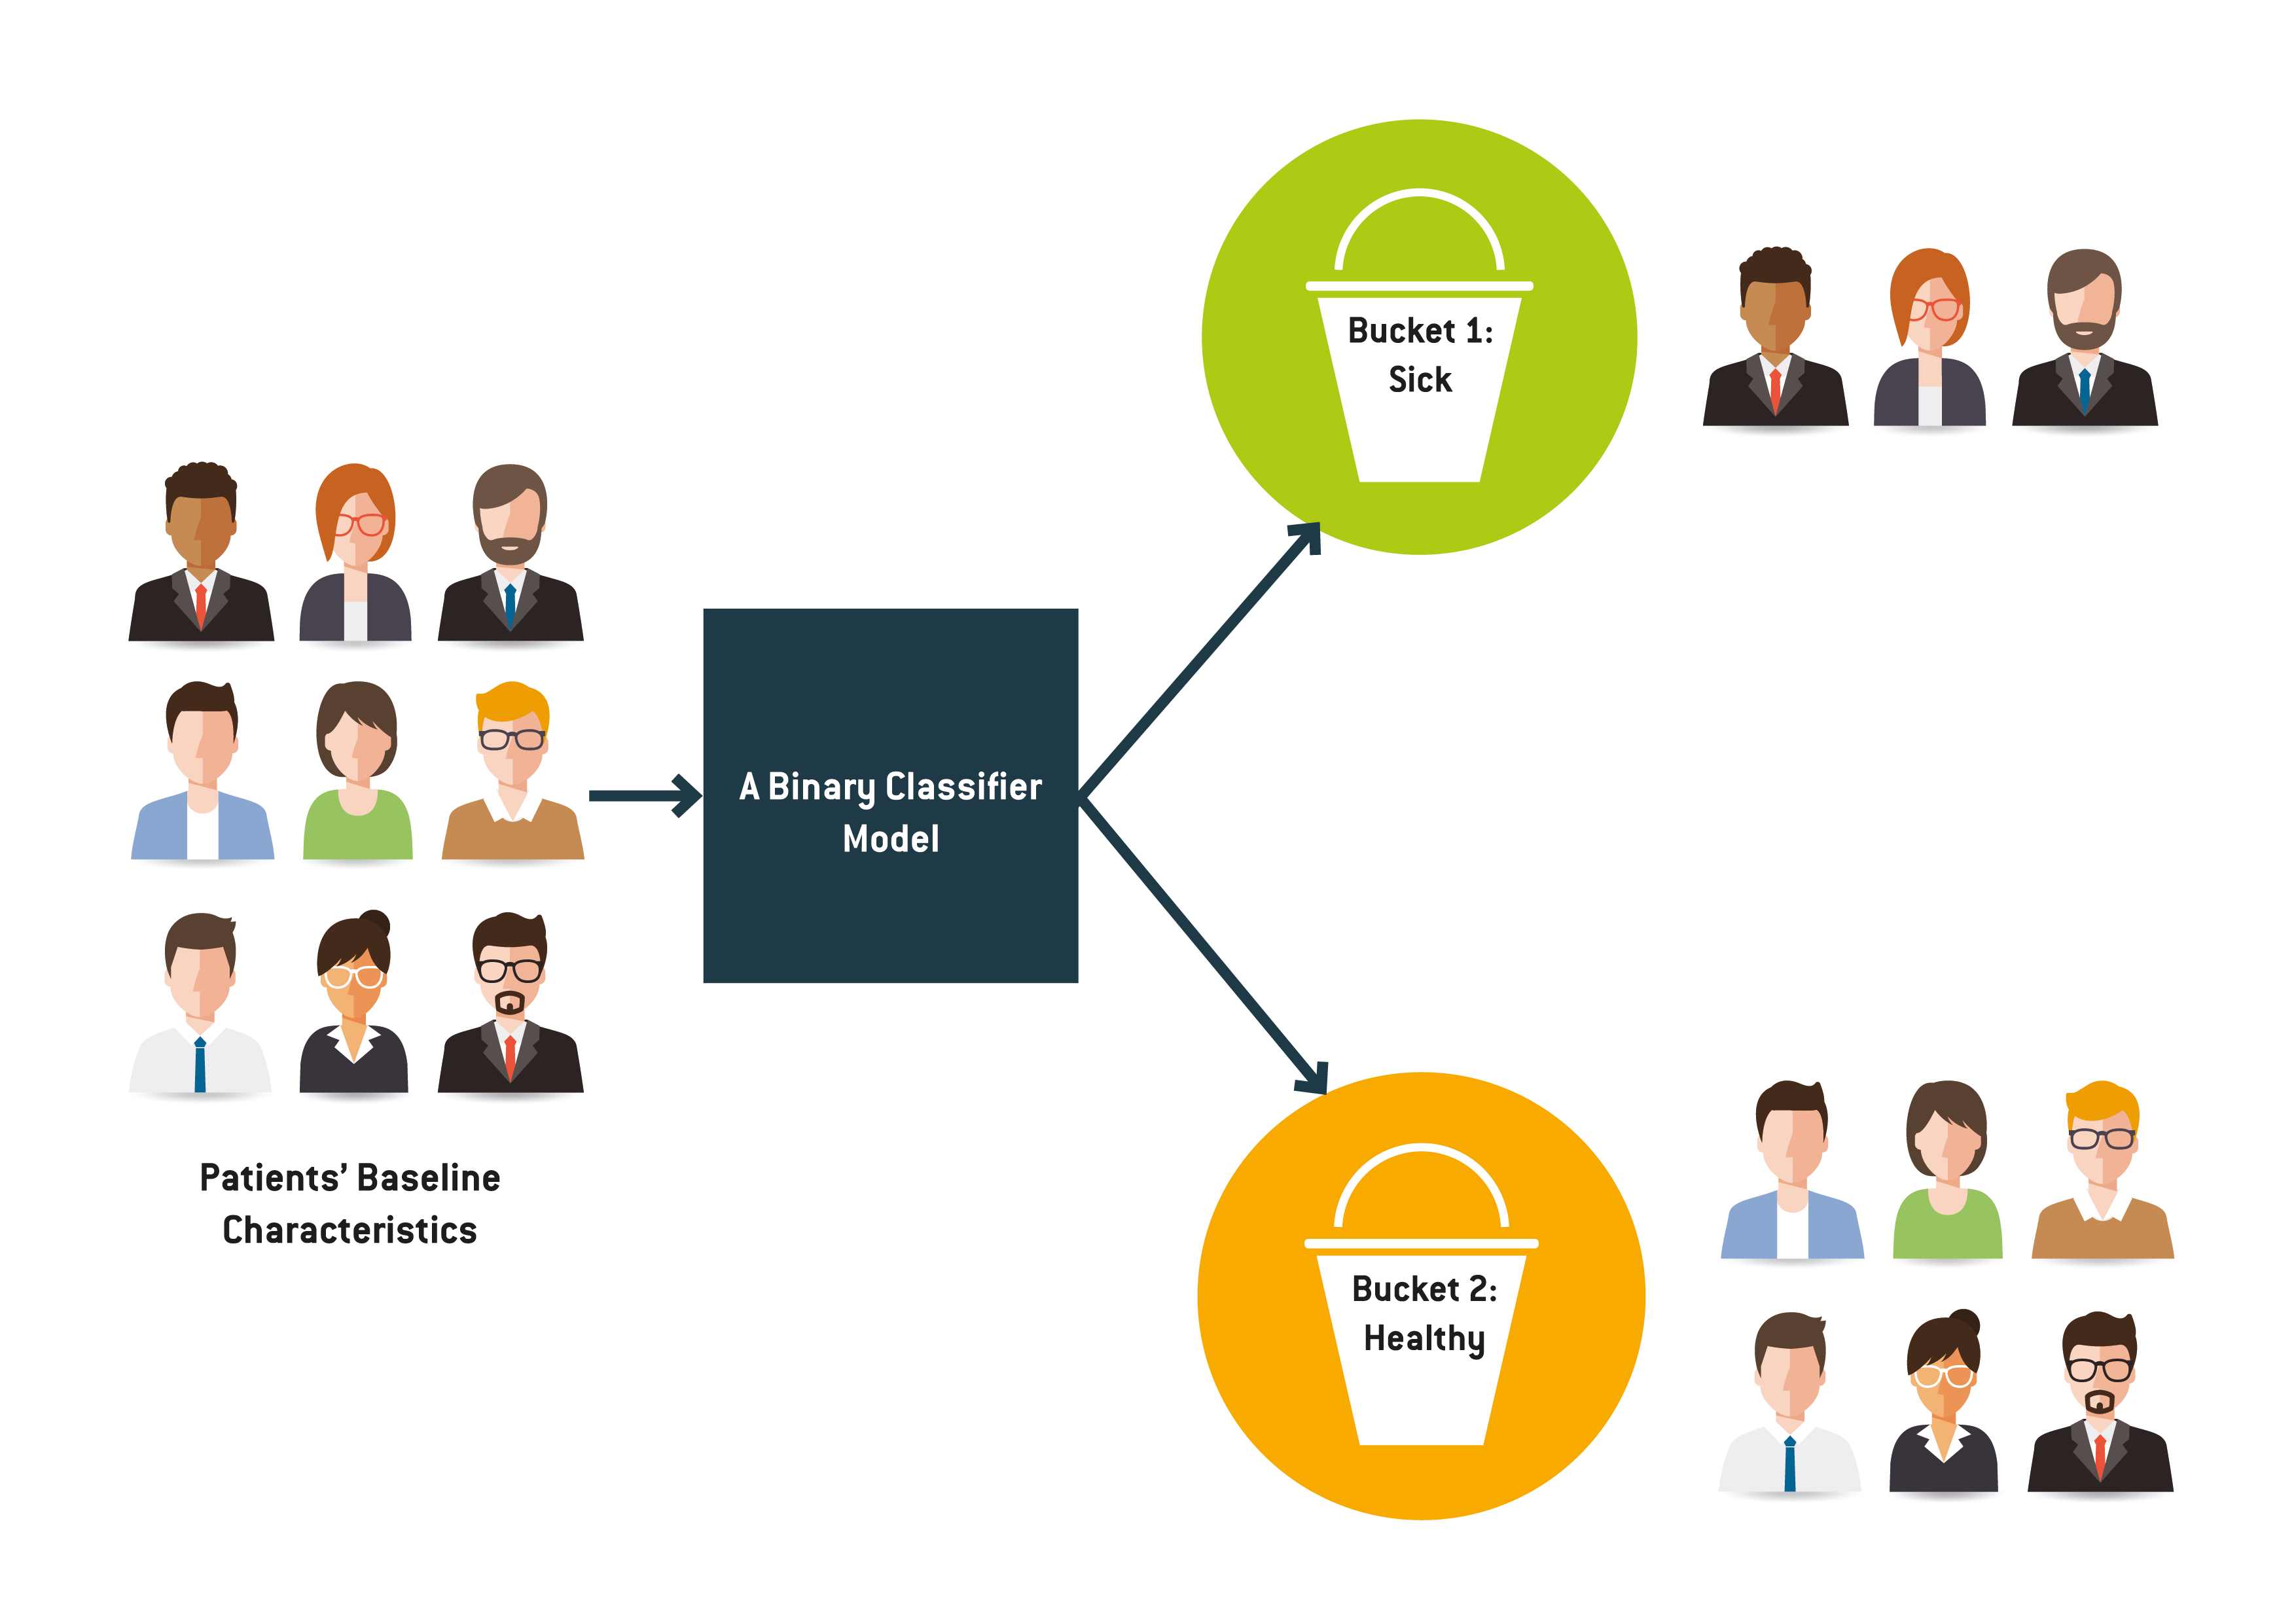
\includegraphics[scale=0.13]{img/Classification/Binary-Classifier-Model.png}
    \centering
    \caption{Classification showcase \parencite{web:S-cubed}}
    \label{fig:classification}
\end{figure}

Code bellow showcase how the following steps were achieved. It looks similar since the idea was for code to be interchangeable regardless of the model.

As mentioned, we first split the data. Split is 80\% training and 20\% testing. For reproducibility reasons, seed is set to specific number (42). In our case, x (train/test) are the features that we use for prediction and y (train/test) being the feature we are trying to predict (what platform user is on).
\begin{listing}[H]
\caption{Split data function}
\begin{minted}{python}
def split_data(data_frame):
    indexer = StringIndexer(inputCol="platformType", 
                            outputCol="label")
    data_frame = indexer.fit(data_frame).transform(data_frame)

    split_ratio = [0.8, 0.2]
    seed = 42
    train_data, test_data = data_frame.randomSplit(split_ratio, 
                                                    seed=seed)

    x_train = train_data.select("platformType").toPandas()
    y_train = train_data.select("label").toPandas()

    x_test = test_data.select("platformType").toPandas()
    y_test = test_data.select("label").toPandas()

    return x_train, x_test, y_train, y_test
\end{minted}
\end{listing}

\newpage
\subsection{Decision tree}

\subsubsection{About}

K-means is a clustering algorithm \parencite{hartigan1979algorithm}. It is one of the more popular algorithms used for clustering. How it usually works is by us providing k (number of clusters) to the algorithm. Our model will then calculate the distance (there are different calculations: Euclidean, Manhattan, etc...) between nodes. Afterwards we can see the ideal number and chose it as our number of clusters.
\newpage
\subsubsection{Implementation}

Implementation is similar to decision tree. We are expecting training data in the function, select platform type as what to predict and vectorise he data. SVM can be optimised as well, grid was used (same as with decision trees) and cross validation was applied as well. At the end, SVM model is returned.
\begin{listing}[H]
\caption{SVM model function}
\begin{minted}{python}
def build_svm_model(x_train, y_train):
    train_data = spark.createDataFrame
                 (pd.concat([x_train, y_train], axis=1))

    platform_indexer = StringIndexer(inputCol="platformType", 
                                     outputCol="indexedLabel")
    train_data = platform_indexer.fit(train_data).transform(train_data)

    assembler = VectorAssembler(inputCols=["indexedLabel"], 
                                outputCol="features")
    train_data = assembler.transform(train_data)

    svm = LinearSVC(featuresCol="features", labelCol="indexedLabel")

    paramGrid = ParamGridBuilder() \
        .addGrid(svm.maxIter, [10, 100]) \
        .addGrid(svm.regParam, [0.1, 0.01]) \
        .build()

    ovr = OneVsRest(classifier=svm)

    evaluator = MulticlassClassificationEvaluator(labelCol="indexedLabel", 
                predictionCol="prediction", metricName="accuracy")
    crossval = CrossValidator(estimator=ovr, estimatorParamMaps=paramGrid, 
                              evaluator=evaluator, numFolds=5)

    cvModel = crossval.fit(train_data)

    return cvModel.bestModel
\end{minted}
\end{listing}




























% \begin{listing}[H]
% \caption{Evaluate SVM model}
% \begin{minted}{python}
% evaluate_model(svm_model, x_test, y_test, file_Path = file_paths_dict["classification"] + "SVM")
% \end{minted}
% \end{listing}

\newpage
\subsubsection{Results}

At the end, we need to evaluate the model in order to get the results. We pass in our model, test data and location where we want results to be saved. The function (that is split into parts 1-4) then evaluates the model and results are available to us.
\begin{listing}[H]
\caption{Evaluate model model function -part 1}
\begin{minted}{python}
def evaluate_model(model, x_test, y_test, file_Path):
    test_data = spark.createDataFrame
                (pd.concat([x_test, y_test], axis=1))

    platform_indexer = StringIndexer(inputCol="platformType", 
                                    outputCol="platformIndex")
    test_data = platform_indexer.fit(test_data).transform(test_data)

    assembler = VectorAssembler(inputCols=["platformIndex"], 
                                outputCol="features")
    test_data = assembler.transform(test_data)

    predictions = model.transform(test_data)

    evaluator = MulticlassClassificationEvaluator(labelCol="label", 
                                        predictionCol="prediction")

    class_labels = test_data.select("label").distinct()
                    .rdd.flatMap(lambda x: x).collect()
    metrics = {}

\end{minted}
\end{listing}

\begin{listing}[H]
\caption{Evaluate model model function -part 2}
\begin{minted}{python}
    for label in class_labels:
        evaluator.setMetricName("accuracy")
        evaluator.setMetricLabel(label)
        accuracy = evaluator.evaluate(predictions)

        evaluator.setMetricName("weightedPrecision")
        evaluator.setMetricLabel(label)
        precision = evaluator.evaluate(predictions)

        evaluator.setMetricName("weightedRecall")
        evaluator.setMetricLabel(label)
        recall = evaluator.evaluate(predictions)

        evaluator.setMetricName("weightedFMeasure")
        evaluator.setMetricLabel(label)
        f1_score = evaluator.evaluate(predictions)

\end{minted}
\end{listing}

\begin{listing}[H]
\caption{Evaluate model model function -part 3}
\begin{minted}{python}
        metrics[label] = {"accuracy": accuracy, "precision": precision, 
                          "recall": recall, "f1-score": f1_score}

    predictionAndLabels = predictions.select("prediction", "label").rdd
    multiclass_metrics = MulticlassMetrics(predictionAndLabels)
    confusion_matrix = multiclass_metrics.confusionMatrix().toArray()

    label_counts = predictionAndLabels.map(lambda x: (x[1], 1))
                   .reduceByKey(lambda x, y: x + y).collectAsMap()
    support = {label: label_counts.get(label, 0) for label in class_labels}

    metrics_table = pd.DataFrame.from_dict(metrics, orient="index")
    print("Metrics per Class:")
    print(metrics_table)

    support_table = pd.DataFrame.from_dict
                    (support, orient="index", columns=["Support"])
    print("Support:")
    print(support_table)

    fig, ax = plt.subplots()
    im = ax.imshow(confusion_matrix, cmap="Blues")

    tick_labels = np.arange(len(class_labels))
    ax.set_xticks(tick_labels)
    ax.set_yticks(tick_labels)
    ax.set_xticklabels(class_labels, rotation=45)
    ax.set_yticklabels(class_labels)
    plt.xlabel("Predicted")
    plt.ylabel("Actual")
\end{minted}
\end{listing}

\begin{listing}[H]
\caption{Evaluate model model function -part 4}
\begin{minted}{python}
    cbar = ax.figure.colorbar(im, ax=ax)
    cbar.ax.set_ylabel("Count", rotation=-90, va="bottom")

    for i in range(len(class_labels)):
        for j in range(len(class_labels)):
            text = ax.text(j, i, int(confusion_matrix[i, j]), 
                           ha="center", va="center", color="w")

    plt.title("Confusion Matrix")
    
    metrics_table.to_csv(file_Path + "/metrics.csv")
    plt.savefig(file_Path + "/confusion_matrix.png")

    plt.close()
\end{minted}
\end{listing}

\begin{figure}[H]
    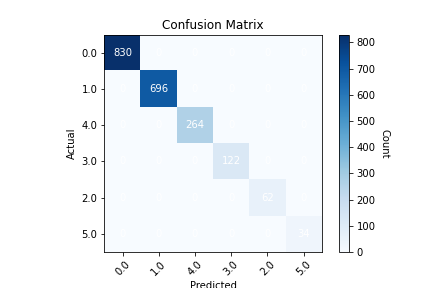
\includegraphics[scale=0.85]{img/Model/Classification/Dtree/confusion_matrix.png}
    \centering
    \caption{Decision tree confusion matrix}
    \label{fig:dtree_confusion_matrix}
\end{figure}
\newpage
\newpage
\subsection{SVM}

\subsubsection{About}

K-means is a clustering algorithm \parencite{hartigan1979algorithm}. It is one of the more popular algorithms used for clustering. How it usually works is by us providing k (number of clusters) to the algorithm. Our model will then calculate the distance (there are different calculations: Euclidean, Manhattan, etc...) between nodes. Afterwards we can see the ideal number and chose it as our number of clusters.
\newpage
\subsubsection{Implementation}

Implementation is similar to decision tree. We are expecting training data in the function, select platform type as what to predict and vectorise he data. SVM can be optimised as well, grid was used (same as with decision trees) and cross validation was applied as well. At the end, SVM model is returned.
\begin{listing}[H]
\caption{SVM model function}
\begin{minted}{python}
def build_svm_model(x_train, y_train):
    train_data = spark.createDataFrame
                 (pd.concat([x_train, y_train], axis=1))

    platform_indexer = StringIndexer(inputCol="platformType", 
                                     outputCol="indexedLabel")
    train_data = platform_indexer.fit(train_data).transform(train_data)

    assembler = VectorAssembler(inputCols=["indexedLabel"], 
                                outputCol="features")
    train_data = assembler.transform(train_data)

    svm = LinearSVC(featuresCol="features", labelCol="indexedLabel")

    paramGrid = ParamGridBuilder() \
        .addGrid(svm.maxIter, [10, 100]) \
        .addGrid(svm.regParam, [0.1, 0.01]) \
        .build()

    ovr = OneVsRest(classifier=svm)

    evaluator = MulticlassClassificationEvaluator(labelCol="indexedLabel", 
                predictionCol="prediction", metricName="accuracy")
    crossval = CrossValidator(estimator=ovr, estimatorParamMaps=paramGrid, 
                              evaluator=evaluator, numFolds=5)

    cvModel = crossval.fit(train_data)

    return cvModel.bestModel
\end{minted}
\end{listing}




























% \begin{listing}[H]
% \caption{Evaluate SVM model}
% \begin{minted}{python}
% evaluate_model(svm_model, x_test, y_test, file_Path = file_paths_dict["classification"] + "SVM")
% \end{minted}
% \end{listing}

\newpage
\subsubsection{Results}

At the end, we need to evaluate the model in order to get the results. We pass in our model, test data and location where we want results to be saved. The function (that is split into parts 1-4) then evaluates the model and results are available to us.
\begin{listing}[H]
\caption{Evaluate model model function -part 1}
\begin{minted}{python}
def evaluate_model(model, x_test, y_test, file_Path):
    test_data = spark.createDataFrame
                (pd.concat([x_test, y_test], axis=1))

    platform_indexer = StringIndexer(inputCol="platformType", 
                                    outputCol="platformIndex")
    test_data = platform_indexer.fit(test_data).transform(test_data)

    assembler = VectorAssembler(inputCols=["platformIndex"], 
                                outputCol="features")
    test_data = assembler.transform(test_data)

    predictions = model.transform(test_data)

    evaluator = MulticlassClassificationEvaluator(labelCol="label", 
                                        predictionCol="prediction")

    class_labels = test_data.select("label").distinct()
                    .rdd.flatMap(lambda x: x).collect()
    metrics = {}

\end{minted}
\end{listing}

\begin{listing}[H]
\caption{Evaluate model model function -part 2}
\begin{minted}{python}
    for label in class_labels:
        evaluator.setMetricName("accuracy")
        evaluator.setMetricLabel(label)
        accuracy = evaluator.evaluate(predictions)

        evaluator.setMetricName("weightedPrecision")
        evaluator.setMetricLabel(label)
        precision = evaluator.evaluate(predictions)

        evaluator.setMetricName("weightedRecall")
        evaluator.setMetricLabel(label)
        recall = evaluator.evaluate(predictions)

        evaluator.setMetricName("weightedFMeasure")
        evaluator.setMetricLabel(label)
        f1_score = evaluator.evaluate(predictions)

\end{minted}
\end{listing}

\begin{listing}[H]
\caption{Evaluate model model function -part 3}
\begin{minted}{python}
        metrics[label] = {"accuracy": accuracy, "precision": precision, 
                          "recall": recall, "f1-score": f1_score}

    predictionAndLabels = predictions.select("prediction", "label").rdd
    multiclass_metrics = MulticlassMetrics(predictionAndLabels)
    confusion_matrix = multiclass_metrics.confusionMatrix().toArray()

    label_counts = predictionAndLabels.map(lambda x: (x[1], 1))
                   .reduceByKey(lambda x, y: x + y).collectAsMap()
    support = {label: label_counts.get(label, 0) for label in class_labels}

    metrics_table = pd.DataFrame.from_dict(metrics, orient="index")
    print("Metrics per Class:")
    print(metrics_table)

    support_table = pd.DataFrame.from_dict
                    (support, orient="index", columns=["Support"])
    print("Support:")
    print(support_table)

    fig, ax = plt.subplots()
    im = ax.imshow(confusion_matrix, cmap="Blues")

    tick_labels = np.arange(len(class_labels))
    ax.set_xticks(tick_labels)
    ax.set_yticks(tick_labels)
    ax.set_xticklabels(class_labels, rotation=45)
    ax.set_yticklabels(class_labels)
    plt.xlabel("Predicted")
    plt.ylabel("Actual")
\end{minted}
\end{listing}

\begin{listing}[H]
\caption{Evaluate model model function -part 4}
\begin{minted}{python}
    cbar = ax.figure.colorbar(im, ax=ax)
    cbar.ax.set_ylabel("Count", rotation=-90, va="bottom")

    for i in range(len(class_labels)):
        for j in range(len(class_labels)):
            text = ax.text(j, i, int(confusion_matrix[i, j]), 
                           ha="center", va="center", color="w")

    plt.title("Confusion Matrix")
    
    metrics_table.to_csv(file_Path + "/metrics.csv")
    plt.savefig(file_Path + "/confusion_matrix.png")

    plt.close()
\end{minted}
\end{listing}

\begin{figure}[H]
    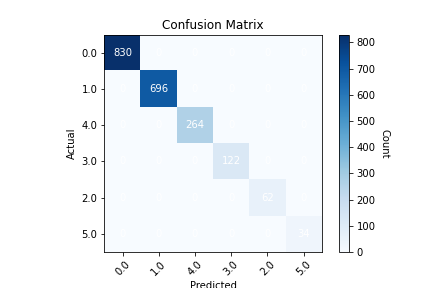
\includegraphics[scale=0.85]{img/Model/Classification/Dtree/confusion_matrix.png}
    \centering
    \caption{Decision tree confusion matrix}
    \label{fig:dtree_confusion_matrix}
\end{figure}
\newpage

\subsection{Execute classification code}

Now that we have the models ready, we can call the code bellow in order to split the data and build models.

\begin{listing}[H]
\caption{Execute the classification functions}
\begin{minted}{python}
x_train, x_test, y_train, y_test = split_data(mega_dataframe)

dt_model = build_decision_tree_model(x_train, y_train)
svm_model = build_svm_model(x_train, y_train)

evaluate_model(dt_model, x_test, y_test, 
file_Path = file_paths_dict["classification"] + "DecisionTree")

evaluate_model(svm_model, x_test, y_test, 
file_Path = file_paths_dict["classification"] + "SVM")

\end{minted}
\end{listing}

Comparing classifications, we can see that our models did not perform the best. Based on the EDA, we know that mobile platform (iphone and android) are ~80\% of the devices used. Since our data is unbalanced, this can be a factor why results are skewed towards one end.
